\chapter{\texorpdfstring{\MakeUppercase{Simplified Example}}{Simplified Example}}

This chapter serves to show a simplified example of the optimization of
the supply air temperature under one given condition. The single example
is studied in detail to elucidate the various competing
components impacting the total power required to satisfy the building
loads. 

For simplicity, a single duct variable air volume system with two
terminal units is assumed. Hot and dry outdoor air conditions are
assumed such that both zones are under a cooling load and there are no
latent load concerns.  

Zone 1 is assumed to have a load of \SI{20000}{\btu\per\hour}, while the
load in Zone 2 is \SI{7344}{\btu\per\hour}. 

The minimum flow setting for the terminal units is \SI{400}{\cfm}. The
room temperature is \SI{72}{\degreeF} and the mixed air temperature is
\SI{80}{\degreeF}.

The fan is assumed to have the following part-load behavior described in
\eqreftext{} \ref{eq:simplifiedExampleFFLP}. The design
flow is chosen so that at a supply temperature of \SI{65}{\degreeF} the
fan is at design flow. 

The design power is chosen so that at the calculated design flow, the
efficiency is \num{0.8} and the pressure rise is \SI{4}{\inchwater}.
Under the chosen conditions, the design flow is \SI{3503}{\cfm}, which
is the resulting flow under the highest tested supply air temperature
\SI{65}{\degreeF}. The resulting design fan power is \SI{2.75}{\hp}. 

\begin{equation}\label{eq:simplifiedExampleFFLP}
    \text{FFLP} = A + \left(1-A\right)(\text{PLR})^{n} =   0.1 + (0.9)(\text{PLR})^{2.5}
\end{equation}
The fan power is 
\begin{equation}
    \dot{W}_{fan} = \text{FFLP} \; \dot{W}_{des} = \text{FFLP}\left(\SI{2.75}{\hp}\right) 
\end{equation}

The required flow for each zone is calculated as 
\begin{equation}
    \flow{z} = \text{MAX} \left( \frac{\heatenergy{z}}{C_{a}
    \left(T_{z} - \sat{}\right)  }, \flow{min}  \right)
\end{equation}
The discharge temperature for each zone is
\begin{equation}
    T_{dis} = T_{z} - \frac{\heatenergy{z}}{C_{a} \; \flow{z}}
\end{equation}
The reheat power is 
\begin{equation}
    \heatenergy{reheat} = C_{a} \flow{z} \left(T_{dis} - \sat{}\right)
\end{equation} 
and the sensible cooling power is 
\begin{equation}\label{eq:sensibleCoolingPower}
    \heatenergy{cool} = C_{a} \flow{tot} \left(\mat{} - \sat{}\right)
\end{equation} 
where \(\flow{tot}\) is the total flow for all the zones. 


\begin{table}
\centering
\caption{Summary of parameters used for simplified example.}
\label{tab:summaryOfParametersForSimplifiedExample}
\begin{tabular}{rl}\toprule
    Parameter              & Value                     \\ \midrule
  System Type              & SDVAV                     \\
  Mixed air temperature    & \SI{80}{\degreeF}         \\
  Zone temperature         & \SI{72}{\degreeF}         \\
  Zone 1 Cooling Load      & \SI{20000}{\btu\per\hour} \\
  Zone 2 Cooling Load      & \SI{7344}{\btu\per\hour}  \\
  Design fan efficiency    & 0.80                      \\
  Design fan pressure rise & \SI{4}{\inchwater}        \\
  Design fan power         & \SI{2.75}{\hp}            \\
  Fan exponent, \(n\)      & 2.5                       \\
  \bottomrule
\end{tabular}
\end{table}

Increasing the supply air temperature has the effect of decreasing
reheat and increasing fan power. Whether the cooling load increases or
decreases depends on several factors. 

For example, during times when there is no reheat, the required flow for
the terminal units is 
\begin{equation}\label{eq:requiredFlow}
    \flow{req} = \frac{\heatenergy{z}}{C_{a} \left(T_{z} - \sat{}\right)}
\end{equation}
%
Substituting \eqreftext{} \ref{eq:requiredFlow} into  
\eqreftext{} \ref{eq:sensibleCoolingPower} results in
%
\begin{equation}
    \heatenergy{cool} = C_{a}  \frac{\heatenergy{z}}{C_{a} \left(T_{z} -
    \sat{}\right)}\left(\mat{} - \sat{}\right) = \heatenergy{z}
    \frac{\mat{} - \sat{}}{T_{z} - \sat{}}
\end{equation}


Of interest is how the sensible cooling power is impacted when
the supply air temperature is increased. To investigate, the derivative
of the sensible cooling power equation is found.

\begin{equation}\label{eq:derivativeOfSensibleCooling}
    \dv{\heatenergy{cool}}{\sat{}} = \heatenergy{z} \frac{\mat{} -
    T_{z}}{\left(T_{z} - \sat{}\right)^{2}}
\end{equation}

What \eqreftext{} \ref{eq:derivativeOfSensibleCooling} shows is the
non-intuitive result that during times of cooling (corresponding to a
positive \(\heatenergy{z}\)) and when the mixed air temperature is
greater than the zone temperature (corresponding to a positive value in
the numerator of \eqreftext{} \ref{eq:derivativeOfSensibleCooling}), that
the sensible cooling power \textit{increases} with increasing supply air
temperature. If a cooling load exists and the mixed air temperature is
less than the zone temperature, then the opposite is true, increasing
the supply air temperature will reduce the required sensible cooling
power.

\figref{} \ref{fig:simplifiedExampleFlow} shows how the supply air flow
changes with regards to the supply air temperature. The zone loads were
chosen in such a way that Zone 1 operates above the minimum flow
setpoint at all times, while Zone 2 is at the minimum flow setpoint at
supply air temperatures less than \SI{57}{\degreeF}. The system uses
reheat at supply air temperatures less than \SI{57}{\degreeF}. 

With the selected system parameters, the total steady state power can be
plotted with respect to the supply air temperature. The total power
function ends up being convex with a minimum at \SI{57}{\degreeF}. 

What is important is the fact that the optimum supply air temperature is
not simply the maximum supply air temperature in the search range. Under
conditions such as the one in the first example, there is a competing
balance between the cooling, reheat, and fan power. It is possible that
the optimization will potentially suggest lowering the supply air
temperature when the conditions are appropriate.

This conclusion is affirmed as well after investigating the impact of
energy cost. The following analysis assumes the fan power uses 
electricity, the cooling is from district chilled water, and the reheat
is from district hot water, and the prices are those from the posted
Texas A\&M Utilities and Energy Services rates for
FY2016\footnote{https://utilities.tamu.edu/2015/08/31/cost-and-fees-for-utility-services-fy2016/}.
The rates are 

\begin{itemize}
    \item Electricity -- \$0.082/kWh \(\approx\) \$24/MMBTU
    \item Chilled Water -- \$15.25/MMBTU
    \item Hot Water -- \$15.03/MMBTU
\end{itemize}

When the cost of electricity is taken into account, the importance of
the relationship between fan power and the supply air temperature is
increased. Chilled water is usually produced with a chiller having a COP
greater than 3 while the electricity is consumed directly for the fan.
When the impact of cost is added, the cost penalty for fan power can grow
significantly at higher supply air temperatures, which can be seen in
\figref{} \ref{fig:simplifiedExampleCost}. 

With cost as the optimization function, the optimal supply air
temperature is reduced from \SI{57}{\degF} to \SI{56.7}{\degF} because
of the higher price of electricity as compared to the district chilled
water and hot water price. 

% Plots/33-SimplifiedExampleFlow/simplifiedExampleFlow.tex
\begin{figure}
\centering
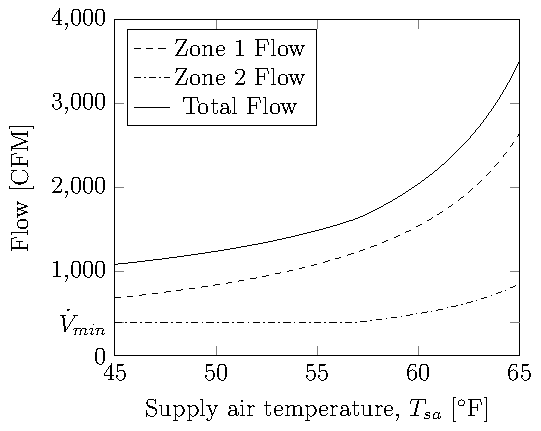
\includegraphics{Plots/33-SimplifiedExampleFlow/simplifiedExampleFlow.pdf}
\caption{Variation of required air flow with respect to different supply
air temperatures.}
\label{fig:simplifiedExampleFlow}
\end{figure}

\newcommand{\variationCaption}[1]{Variation of total #1 with respect to
different supply air temperatures, using \SI{80}{\degreeF} as the mixed
air temperature. }

\begin{figure}
\centering
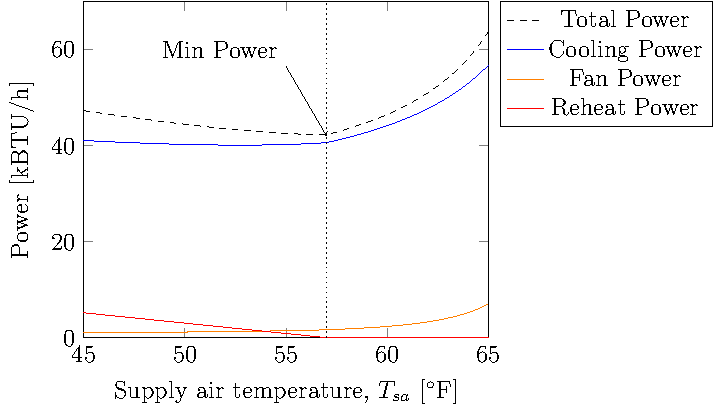
\includegraphics{Plots/32-SimplifiedExample/simplifiedExample.pdf}
\caption{\variationCaption{power}}
\label{fig:simplifiedExamplePower}
\end{figure}

\begin{figure}
\centering
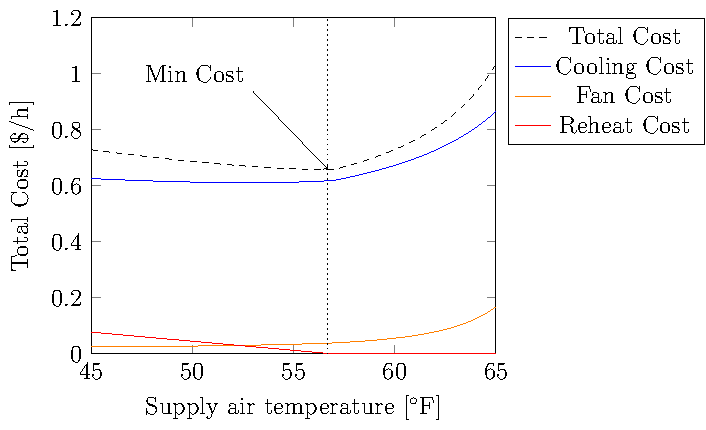
\includegraphics{Plots/35-SimplifiedExampleCostHighMAT/simplifiedExampleCostHighMAT.pdf}
\caption{\variationCaption{cost}}
\label{fig:simplifiedExampleCost}
\end{figure}

If the mixed air temperature is reduced from \SI{80}{\degreeF} to
\SI{65}{\degreeF}, the resulting total power function changes
drastically. The required flow rates for each of the zones remains the
same, along with the fan power and the reheat power. Since the mixed air
temperature is less than the zone temperature, the slope of the sensible
cooling power function is always negative, since the numerator in
\eqreftext{} \ref{eq:derivativeOfSensibleCooling} is negative. The
result of this is that the minimum total power occurs at the maximum of
the supply air temperature search range.   

\newcommand{\variationCaptionLowMAT}[1]{Variation of total #1 with respect to different supply air
temperatures, with a mixed air temperature of \SI{65}{\degreeF} instead
of the original \SI{80}{\degreeF}.}

\begin{figure}
\centering
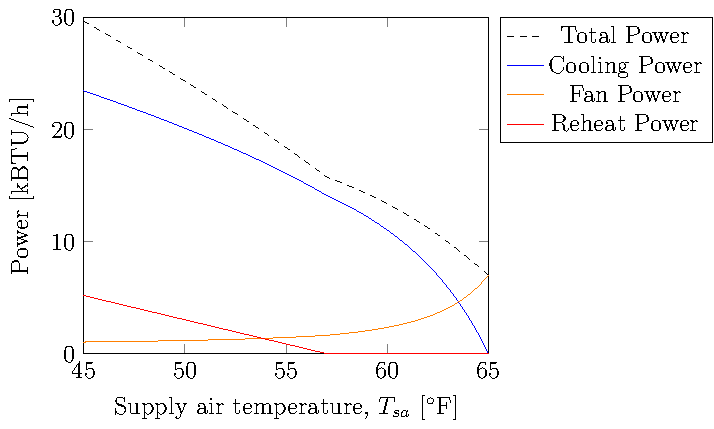
\includegraphics{Plots/34-SimplifiedExampleLowerMAT/simplifiedExampleLowerMAT.pdf}
\caption{\variationCaptionLowMAT{power}}
\label{fig:simplifiedExamplePowerLowerMAT}
\end{figure}

\begin{figure}
\centering
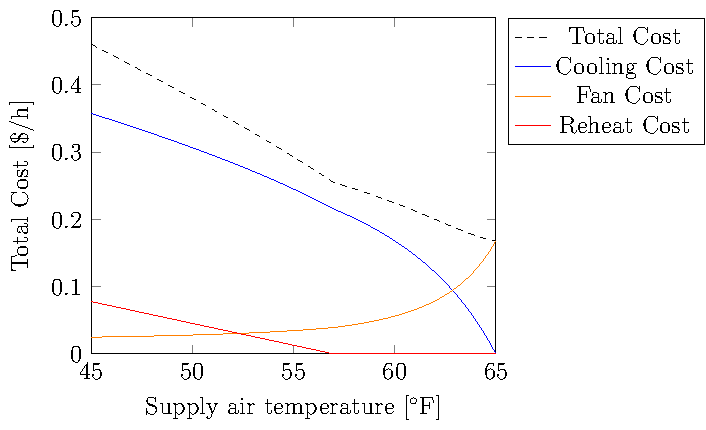
\includegraphics{Plots/36-SimplifiedExampleCostLowerMAT/simplifiedExampleCostLowMAT.pdf}
\caption{\variationCaptionLowMAT{cost}}
\label{fig:simplifiedExampleCostLowerMAT}
\end{figure}


\section{Function Analysis}

While attempting to optimize an AHU system, it is helpful to understand
how the supply temperature affects all portions of the total power. The
analysis in this section relates to a simplified single duct variable
air volume system, with terminal units having a traditional control
sequence, initiating reheat at a constant minimum flow. 

The investigation is going to assume that at a given supply air
temperature, a certain amount of terminal units are going to be in
reheat mode, operating at minimum flow, while the others are operating
in cooling mode. The total flow for the system is then 
%
\begin{equation}
    \flow{tot} = \flow{min,1} + \flow{min,2} + \ldots +
    \frac{\heatenergy{z,3}}{C_{a} \left(T_{z,3} - \sat{}\right) } +
    \frac{\heatenergy{z,4}}{C_{a} \left(T_{z,4} - \sat{}\right) } +
    \ldots
\end{equation}
%
If the zone temperatures, \(T_{z}\) are all the same, then the terms
related to zones in cooling can be combined. All the flows related to
the zones operating at minimum flow can also be combined.
\begin{equation}
    \flow{tot} = \sum \flow{mins} + \frac{\sum \heatenergy{z,tot}}{C_{a}
    \left(T_{z} - \sat{}\right) } 
\end{equation}
%
For clarity, for the rest of the derivations, the sum will be assumed,
and the system can just be imagined as a combined, two terminal unit
system, in which one of the units is operating at minimum flow and the
other terminal unit is in cooling mode. 

\subsection{Sensible Cooling Power}

\newcommand{\totalFlow}{\flow{min} + \frac{\heatenergy{z}}{C_{a}\left(T_{z}-\sat{}\right)}}
The total sensible cooling power, \(\heatenergy{c,s}\), is
\begin{equation}\label{eq:sensiblePowerTotal}
    \heatenergy{c,s} =  C_{a} \flow{tot} \left(\mat{}-\sat{}\right)
\end{equation}
where \(\flow{tot}\) is 
\begin{equation}\label{eq:totalFlowSimpleExample}
    \flow{tot} = \totalFlow{}
\end{equation}
There are two different assumptions that can be made relating to the
outside air flow. The first assumption is that the outside air flow is
constant, while the second assumption is that the fraction of outside
air is constant. 

\subsubsection{Constant Outside Air Flow} 

If the amount of outside air flow is constant at \(\flow{oa}\), and the
return air temperature is assumed to be equal to the zone temperature,
then the mixed air temperature can be estimated as 
\begin{equation}\label{eq:mixedAirConstantOAFlow}
    \mat{} = \frac{\oat{} \flow{oa} + \left(\flow{tot}-\flow{oa}\right) T_{z}}{\flow{tot}} 
\end{equation}
Substituting \eqreftext{} \ref{eq:mixedAirConstantOAFlow} into
\ref{eq:sensiblePowerTotal} results in
\begin{equation}
    \heatenergy{c,s} = C_{a} \flow{tot} \left[ \frac{\oat{} \flow{oa} +
    \left(\flow{tot}-\flow{oa}\right) T_{z}}{\flow{tot}}  - \sat{}  \right]
\end{equation}
Rearranging results in
\begin{equation}
    \heatenergy{c,s} = C_{a} \left[ \flow{oa} \left(\oat{} - T_{z}\right) + \flow{tot}
    \left(T_{z} - \sat{}\right)  \right]
\end{equation}
When \(\flow{tot}\) is replaced with \eqreftext{}
\ref{eq:totalFlowSimpleExample}, the (\(T_{z}-\sat{}\)) term cancels
out, and the final form for \(\heatenergy{c,s}\) is 
\begin{equation}\label{eq:sensiblePowerConstantOAFlow}
    \heatenergy{c,s} = \heatenergy{z} + C_{a} \flow{oa}
    \left(\oat{}-T_{z}\right)  + C_{a} \flow{min} \left(T_{z} - \sat{} \right)
\end{equation}
The portion of \eqreftext{} \ref{eq:sensiblePowerConstantOAFlow} that
depends on the supply air temperature is related to the minimum flow, or
the zones that are in reheat. If no zones were in reheat, then the
sensible cooling power would not depend on the supply air temperature. 

The derivative of \eqreftext{} \ref{eq:sensiblePowerConstantOAFlow} is
\begin{equation}
    \dv{\heatenergy{c,s}}{\sat{}} = -C_{a} \flow{min} 
\end{equation}
which means that the sensible cooling power decreases as the supply air
temperature is raised at a constant slope. 

%\eqreftext{}
%\ref{eq:sensiblePowerConstantOAFlow} could also have been derived using
%an energy balance which included both the zones and the air handling
%unit. 

\subsubsection{Constant Outside Air Fraction}

If the percentage of outside air is held constant instead of the flow,
the analysis of the sensible cooling load changes. If the outside air
fraction, \(X_{oa}\) is constant, and the return air temperature is assumed to be
equal to the zone temperature, an estimation of the mixed air temperature is
\begin{equation}\label{eq:mixedAirTempConstantOAF}
    \mat{} = T_{z} + X_{oa} \left(\oat{} - T_{z}\right)
\end{equation}
Substituting \eqreftext{} \ref{eq:mixedAirTempConstantOAF} into
\ref{eq:sensiblePowerTotal} and expanding \(\flow{tot}\) results in
\begin{equation}\label{eq:sensibleCoolingPowerExpandedConstantOAF}
    \heatenergy{c,s} = C_{a} \left[ \totalFlow{} \right] \left[ T_{z} + X_{oa} \left(\oat{} - T_{z}\right) - \sat{}  \right]
\end{equation}
Taking the derivative of \eqreftext{}
\ref{eq:sensibleCoolingPowerExpandedConstantOAF} with respect to
\(\sat{}\) results in
\begin{equation}\label{eq:firstDerivativeSensible}
    \dv{\heatenergy{c,s}}{\sat{}} = \frac{\heatenergy{z} (\oat{}-T_{z})
    X_{oa}}{(\sat{}-T_{z})^2}-C_{a} \flow{min}
\end{equation}

If the outdoor air temperature is less than the zone temperature, the
numerator of the first term becomes negative and the second term is
always negative, so \(\dv{\heatenergy{c,s}}{\sat{}}\) will be negative.
\(\heatenergy{z}\) is assumed to be a cooling load and therefore is
always a positive value. 

A negative slope for \(\dv{\heatenergy{c,s}}{\sat{}}\) implies that the
total sensible cooling power decreases as the supply air temperature is
raised. However, if the outdoor air temperature is greater than the zone
temperature, and the magnitude of the first term is greater than the
contribution from the second term relating to the terminal units that
are in reheat, this slope can become positive, implying the opposite
case. This is similar to the case described at the beginning of this
chapter. 

The second derivative of the function is taken to determine the
curvature of the function. Taking the derivative of \eqreftext{}
\ref{eq:firstDerivativeSensible} results in
\begin{equation}
    \dv[2]{\heatenergy{c,s}}{\sat{}} = \frac{2 \heatenergy{z}
    \left(T_{oa}-T_z\right) X_{oa} }{\left(T_z-\sat{}\right)^3}
\end{equation}
The sign of \(\dv[2]{\heatenergy{c,s}}{\sat{}}\) is solely determined by
the sign of \((\oat{}-\sat{})\) since \(\heatenergy{z}\) is positive
and \(T_z > \sat{} \). This means that if the outdoor air temperature is
greater than the zone temperature, there can be a power penalty for
raising the supply air temperature, and this penalty gets worse as the
supply air temperature is increased.  


\subsection{Latent Cooling Power}

The total latent cooling power, \(\heatenergy{c,l}\), is 
\begin{equation}\label{eq:latentCoolingPower}
   \heatenergy{c,l} = H \left(\totalFlow \right) \left( \omega_{ma} -
   \omega_{sa} \right) 
\end{equation}
where \(H\) is a volumetric heat of vaporization for water and \(\omega_{sa}\)
is the saturation humidity ratio at a given supply air temperature, which means
that it is a function of the supply air temperature.  For this analysis it is
assumed that a latent load does exist and \(\omega_{ma} >
\omega_{sa}(\sat{})\). If \(\omega_{sat}(\sat{}) > \omega_{ma}\), then
the latent load is zero and all its derivatives are zero as well.

Taking the derivative of \eqreftext{} \ref{eq:latentCoolingPower} results in
\begin{equation}\label{eq:firstDerivativeLatentPower}
    \dv{\heatenergy{c,l}}{\sat{}} = \frac{H \heatenergy{z} \left(\omega_{ma} -\omega_{sa} \right)}{C_{a} (T_{z}-\sat{})^2} 
    -H \dv{\omega_{sa}}{\sat{}} \left(\frac{\heatenergy{z}}{C_{a} (T_{z}-\sat{})}+\flow{min}\right) 
\end{equation}

At this point, it is helpful to examine the relationship between the
saturated humidity ratio versus temperature. 

As a useful approximation, the relationship between the saturation
humidity ratio and temperature can be described by a third order
polynomial in a restricted range. Over the range of \SI{20}{\degreeF} to
\SI{110}{\degreeF}, the saturation humidity ratio at sea level pressure
can be approximated by
    %\omega_{sa} = 8.06351798049242e-08 T^3 -7.22842996070465e-06 T^2 + 0.000384513331591622 T   -0.00358762959892911
\begin{multline}
    \omega_{sa} = \left(8.0635 \times 10^{-8}\right) T^3 \\ 
    - \left(7.2284 \times 10^{-6}\right)  T^2 + \left(3.8451\times 10^{-4}\right) T \\
    -  3.5876\times 10^{-3}
\end{multline}
where \(T\) is in units of \si{\degreeF}. The maximum absolute error in
this range is approximately \num[group-separator={ }]{0.00058787} and the median absolute
deviation is \num[group-separator={ }]{0.000164}. A plot of the fit
versus the more explicit computation is shown in \figref{}
\ref{fig:saturationHumidityRatioVsTemperature}. The first and second
derivative of \(\omega_{sa}\) is shown in \figref{}
\ref{fig:firstDeriviativeSaturationHumidityRatioVsTemperature} and
\figref{}
\ref{fig:secondDeriviativeSaturationHumidityRatioVsTemperature}. It is
clear that the first derivative is always positive and the second
derivative is positive after \SI{30}{\degreeF}.

\begin{figure}
\centering
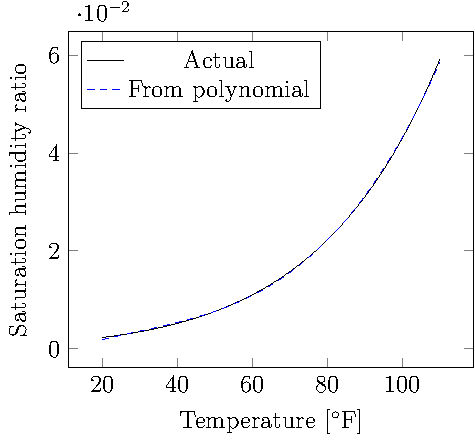
\includegraphics{Plots/44-SaturatedHumidityVsTemperature/saturationHumidityVsTemperature.pdf}
\caption{Saturation humidity ratio versus temperature.}
\label{fig:saturationHumidityRatioVsTemperature}
\end{figure}


% Plots/45-FirstDerivativeSaturatedHumidityVsTemperature/firstDerivativeSaturatedHumidity.tex
\begin{figure}
\centering
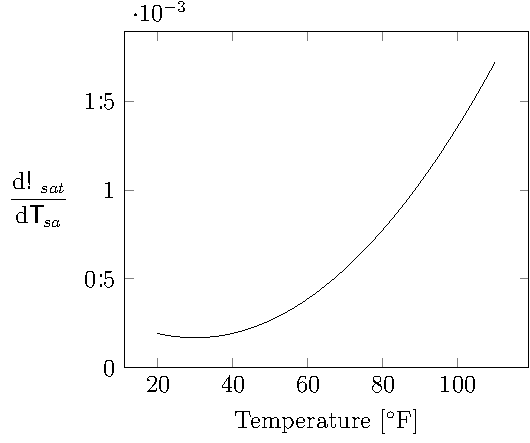
\includegraphics{Plots/45-FirstDerivativeSaturatedHumidityVsTemperature/firstDerivativeSaturatedHumidity.pdf}
\caption{First derivative of the saturation humidity ratio versus temperature.}
\label{fig:firstDeriviativeSaturationHumidityRatioVsTemperature}
\end{figure}

\begin{figure}
\centering
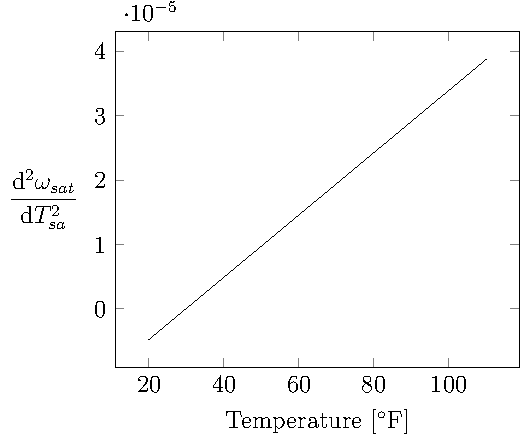
\includegraphics{Plots/46-SecondDerivativeSaturatedHumidityVsTemperature/secondDerivativeSaturatedHumidity.pdf}
\caption{Second derivative of the saturation humidity ratio versus temperature.}
\label{fig:secondDeriviativeSaturationHumidityRatioVsTemperature}
\end{figure}

With this information about the derivatives of the saturation humidity
ratio, it's clear that the first term in \eqreftext{}
\ref{eq:firstDerivativeLatentPower} is positive, while the second term
is negative. Through experimentation with typical values for the
parameters, this results in a negative slope. 

The second derivative of the saturation humidity ratio with respect to
supply air temperature is
\begin{equation}
    \dv[2]{\heatenergy{c,l}}{\sat{}}  =  -H \dv[2]{\omega_{sa}}{\sat{}} \left(\frac{\heatenergy{z}}{C_{a}
            (T_{z}-\sat{})}+\flow{min}\right)+\frac{2 H
            \heatenergy{z} (\omega_{ma}-\omega_{sa})}{C_{a}
            (T_{z}-\sat{})^3}-\frac{2 H \heatenergy{z}
        \dv{\omega_{sa}}{\sat{}}}{C_{a} (T_{z}-\sat{})^2}
\end{equation}
From inspection, it is difficult to discern whether this second
derivative is typically positive or negative. From experimentation it
has been found that this value is typically negative, resulting in
rapidly increasing savings with regards to the latent cooling power by
increasing the supply air temperature. 

\subsection{Fan Power}

The total fan power is
\begin{equation}\label{eq:fanPowerForDerivative}
    \power{fan} = \left(A + \left(1-A\right)\left(\frac{\totalFlow{}}{\flow{des}}\right)^{n}\right) \power{des}
\end{equation}
The first derivative of the fan power with respect to supply air
temperature is
\begin{equation}
    \dv{\power{fan}}{\sat{}} =\frac{(1-A) n \heatenergy{z} \power{des}
    \left(\frac{\frac{\heatenergy{z}}{C_{a}
(T_{z}-\sat{})}+\flow{min}}{\flow{des}}\right)^{n-1}}{C_{a} \flow{des}
(T_{z}-\sat{})^2} 
\end{equation}
or replacing with the definition of the part load ratio (PLR),
\begin{equation}
    \dv{\power{fan}}{\sat{}} =\frac{(1-A) n \heatenergy{z} \power{des}
    \left( \text{PLR} \right)^{n-1}}{C_{a} \flow{des}
(T_{z}-\sat{})^2} 
\end{equation}
The first derivative is always positive, as expected. As the supply air
temperature is increased, it will require an increase in fan power.

The second derivative of fan power with respect to supply air
temperature is 
\begin{equation}\label{eq:secondDerivativeFanPower}
    \frac{\left(1-A\right) n \heatenergy{z} \power{des} \left(2 C_{a}
            \flow{min}
                    (T_{z}-\sat{})+(n+1) \heatenergy{z}\right) \left(\frac{\frac{\heatenergy{z}}{C_{a}
                (T_{z}-\sat{})}+\flow{min}}{\flow{des}}\right)^n}{\left(T_{z}-\sat{}\right)^2
            \left(C_{a} \flow{min} \left(T_{z}-\sat{}\right)+\heatenergy{z}\right)^2}
\end{equation}
While \eqreftext{} \ref{eq:secondDerivativeFanPower} is complicated and
has many terms, it is strictly positive, which means that the fan power
penalty from raising the supply air temperature increases with
increasing supply air temperature, an expected result. 

\subsection{Reheat Power}

Of the four major components (sensible cooling, latent cooling, fan, and
reheat), reheat power is the most straightforward to analyze. The total
reheat power has contributions from only the zones that are at minimum
flow and is equal to
\begin{equation}
    \heatenergy{r} = C_{a} \flow{min} \left(T_{dis} - \sat{} \right)
\end{equation}
The required discharge temperature is
\begin{equation}
    T_{dis} = T_{z} - \frac{\heatenergy{z}}{C_{a} \flow{min} }
\end{equation}
Substituting the equation for \(T_{dis}\) into the total reheat power
equation results in
\begin{equation}
    \heatenergy{r} = C_{a} \flow{min} \left(T_{z} - \frac{\heatenergy{z}}{C_{a} \flow{min} } - \sat{} \right) 
\end{equation}
The derivative of the reheat power with respect to the supply air
temperature is just
\begin{equation}
    \dv{\heatenergy{r}}{\sat{}} = -C_{a} \flow{min}
\end{equation}
and the second derivative is 0. 

As expected, when the supply air temperature is raised, the reheat power
decreases, and this decrease is linear, different from the other
components which have had a non-zero second derivative, implying
curvature. 

\subsection{Summary}

The following derivations were for a simplified model of a single duct
variable air volume system. The zone temperatures from each zone were
assumed to be equal which allowed for the zones in reheat and the zones
not in reheat to be combined. The traditional control sequence analyzed
here is also falling out of favor, with dual-maximum logic becoming more
popular. The analysis is also only valid as long as a box does not
transition from cooling to reheat in the span of supply air temperatures
analyzed. 

Even with these simplifications, it is clear that analytically solving
for the optimal supply air temperature using traditional calculus
techniques would be a difficult endeavor. Even in the simplified model, there are
many interactions between the four major contributors to energy use. The
exercise showed that fan, reheat, and latent portions have a
straightforward dependence on the supply air temperature. However, it
was shown that the sensible cooling power can have its relationship
flipped depending on the relationship between the mixed air temperature
and the zone temperatures. 

